\documentclass[titlepage,a4paper]{article}

\usepackage{a4wide}
\usepackage[colorlinks=true,linkcolor=black,urlcolor=blue,bookmarksopen=true]{hyperref}
\usepackage{amsmath}
\usepackage{bookmark}
\usepackage{fancyhdr}
\usepackage[spanish]{babel}
\usepackage[utf8]{inputenc}
\usepackage[T1]{fontenc}
\usepackage{graphicx}
\usepackage{float}

\pagestyle{fancy} % Encabezado y pie de página
\fancyhf{}
\fancyhead[L]{TP1S - Max Mustermann}
\fancyhead[R]{Algoritmos y Programación III - FIUBA}
\renewcommand{\headrulewidth}{0.4pt}
\fancyfoot[C]{\thepage}
\renewcommand{\footrulewidth}{0.4pt}

\begin{document}
\begin{titlepage} % Carátula
	\hfill
\includegraphics[width=6cm]{logofiuba.jpg}
    \centering
    \vfill
    \Huge \textbf{Trabajo Práctico 2 - Algohoot\\ Primera Entrega}
    \vskip2cm
    \Large [7507/9502] Algoritmos y Programación III\\
    Curso 1\\ % Curso 1 para el de la tarde y 2 para el de la noche
    Primer cuatrimestre de 2020 
    \vfill
    \begin{tabular}{ | l | l | } % Datos del alumno
      \hline
      Alumno: & Rosenblatt \\ \hline
      Número de padrón: & 123456 \\ \hline
      Email: & mmustermann@fi.uba.ar \\ \hline
  	\end{tabular}
    \vfill
    \vfill
\end{titlepage}

\tableofcontents % Índice general
\newpage

\section{Introducción}\label{sec:intro}
El presente informe reune la documentación de la solución del segundo trabajo práctico de la materia Algoritmos y Programación III que consiste en implementar el juego de trivia Kahoot, denominado por nosotros como Algohoot, utilizando los conceptos del paradigma de la orientación a objetos vistos hasta ahora en el curso.

\section{Supuestos}\label{sec:supuestos}
% Deberá contener explicaciones de cada uno de los supuestos que el alumno haya tenido que adoptar a partir de situaciones que no estén contempladas en la especificación.

\subsection{Puntaje Negativo}

Un jugador admite puntaje negativo si responde mal una pregunta con penalidad y tiene puntaje nulo. 

\section{Diagramas de Clases}\label{sec:diagramasdeclase}
% Uno o varios diagramas de clases mostrando las relaciones estáticas entre las clases.  Puede agregarse todo el texto necesario para aclarar y explicar su diseño. Recuerden que la idea de todo el documento es que quede documentado y entendible cómo está implementada la solución.

Juego será un singleton, es decir, solo puede ser instanciada una vez. Está conformado por dos jugadores y una o más preguntas. Cada jugador responderá cuando su turno lo indique, creando así una instancia de Respuesta por cada pregunta respondida. Las preguntas se clasificarán por:\\


\begin{tabular}{l}
Tipo: "Verdadero o Falso"$ $ y "Multiple Choice" $ $(hasta el momento).\\
Modalidad: Clásica, con puntaje Parcial y con Penalidad.\\\\
\end{tabular}

Por cada turno, la pregunta en curso recibirá una lista de respuestas emitidas por cada jugador. \\

A continuación detallaremos como se relacionan las clases:

\begin{enumerate}
\item A
\item B
\item C
\end{enumerate}


\begin{figure}[H]
\centering
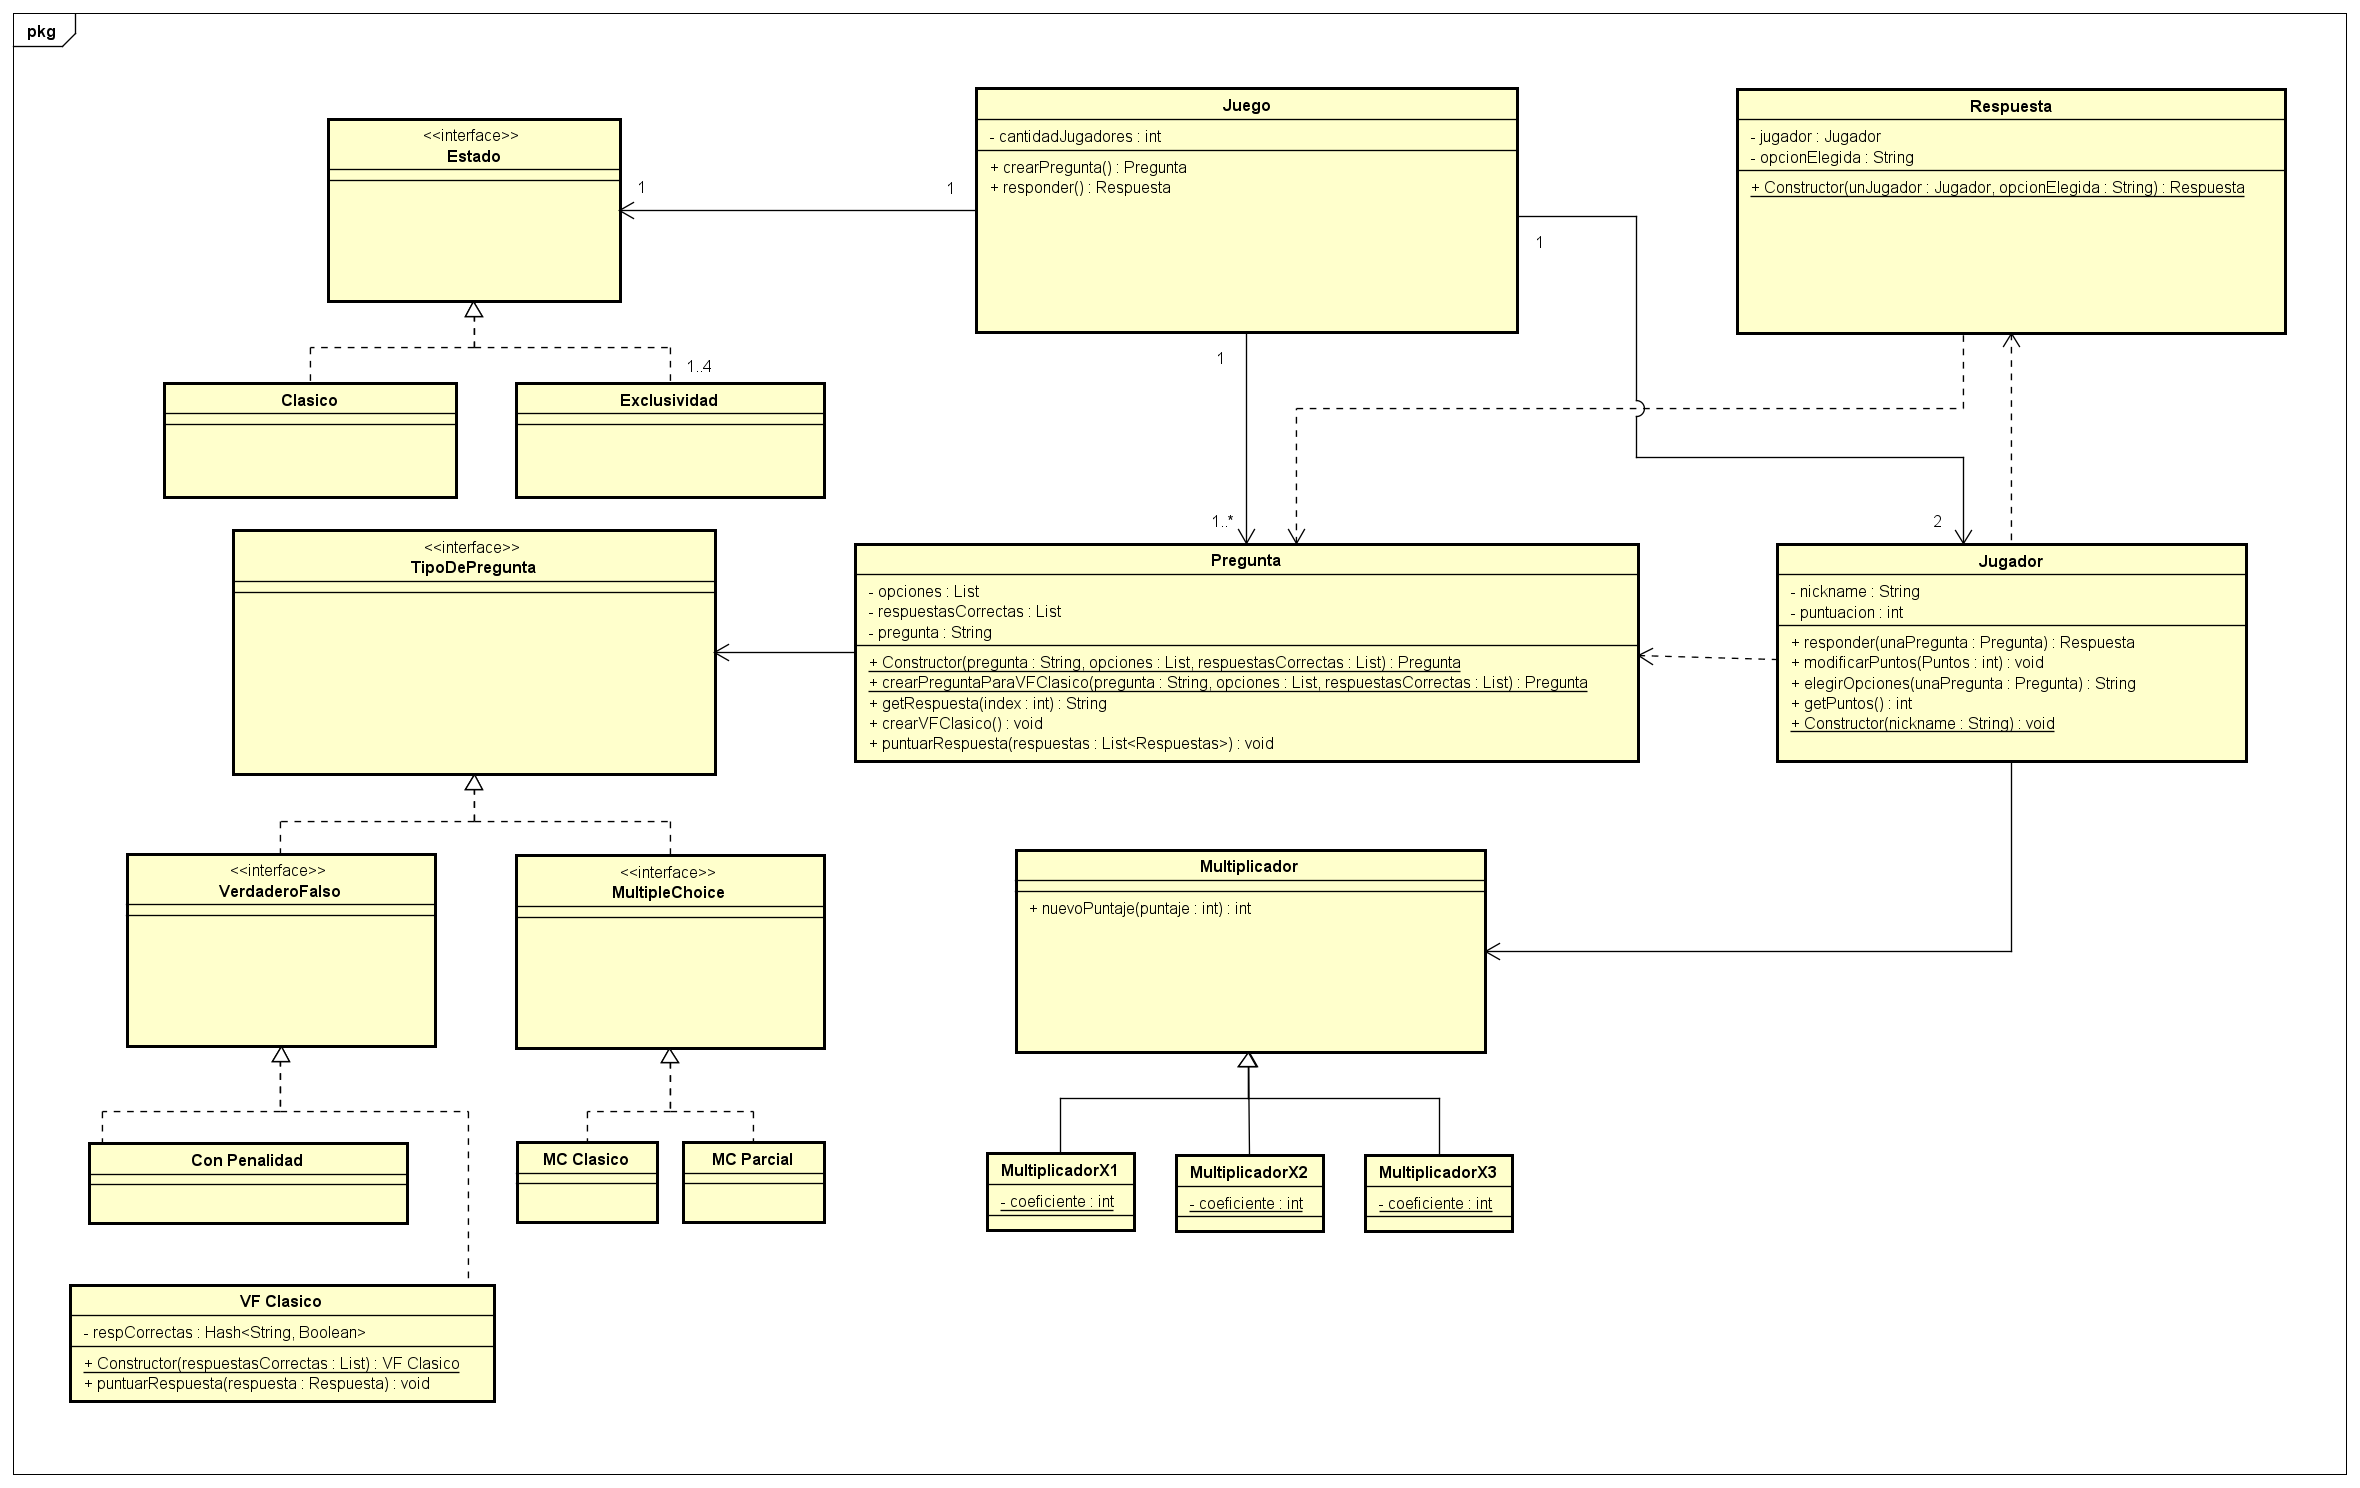
\includegraphics[width=0.8\textwidth]{/home/niyo/Algoritmos y Programación/Kahoot-TP2/resources/diagramas_UML/1. UML Clases (Inicial).png}
\caption{\label{fig:class01}Diagrama del Sudoku.}
\end{figure}

\section{Diagramas de Secuencia}

COMPLETAR


\section{Diagrama de Paquetes}
% Explicación concisa del diseño general del trabajo.

Casi seguro que no se pide

\section{Diagramas de Estados}
% Explicación concisa del diseño general del trabajo.

Casi seguro que no se pide

\section{Detalles de implementación}
% Explicaciones sobre la implementación interna de algunas clases que consideren que puedan llegar a resultar interesantes.

COMPLETAR

\section{Excepciones}
% Explicación de cada una de las excepciones creadas y con qué fin fueron creadas.

\begin{description}
\item[Exception] COMPLETAR
\end{description}

\end{document}